\section{High Level Design}
Our implementation required 8 \texttt{GAL22V10} chips. 6 of these chips were
MOD-n counters which were modified to suit the purpose of providing particular
traffic flows and their timings. The remaining 2 were overarching control chips
to provide inter-flow logic based on sensor inputs and current flow state. A
block diagram is provided in figure \ref{fig:overall-design}.

The diagram does not explain everything in the design, those more complex
details are provided in their relevant section later in this document. The
``Minor Controller'' was necessary due to a limitation in the number of inputs
in the main controller. This diagram does not indicate anything to do with pin
positions, rather, it shows the conceptual blocks of the design. Controller
outputs are indicated in red, and Controller inputs are indicated in green. Flow
chip colours are vice-versa.

\begin{figure*}[!t]
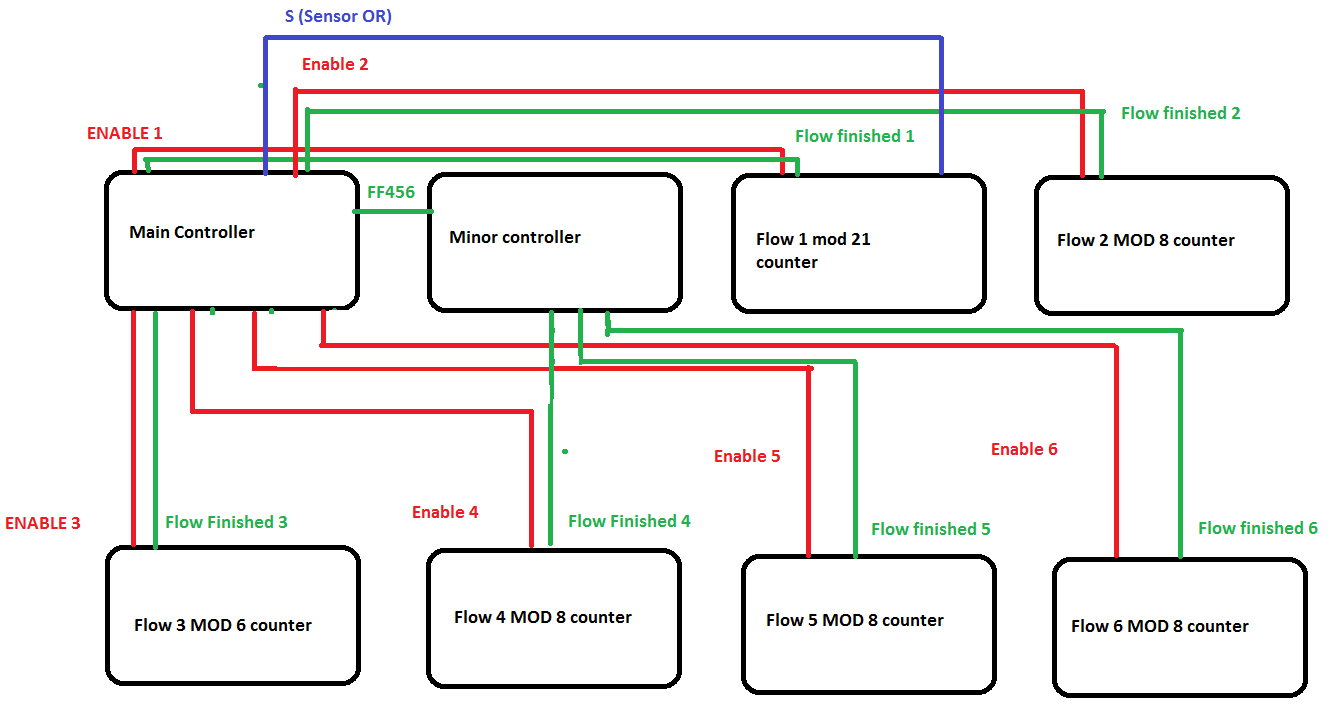
\includegraphics[width=\linewidth]{img/LJNpzV.png}
\caption{High level design block diagram}
\label{fig:overall-design}
\end{figure*}

The basic idea of this design is the following: The ``Main Controller'' is in
charge of which flow is on and which is off, it can enable them through the \ENX
(\texttt{ENABLE} flow $X$) line which it puts as \HIGH whenever it wants that
flow to begin ticking. Once that flow has completed its timing (and thus
relieved the traffic from that side) it will then raise the \FFX (Flow
Finished X) to indicate to the main controller that it has completed its cycle,
at which point the main controller will change that \ENX to \LOW to switch off
that flow, it then evaluates the sensor inputs and decides which flow to enable
next, which it will then enable by making that flows Enable line high, and so
on. This is the basic logic that governs the progression between the flows and
how it deals with traffic. \textbf{Note:} the \ENX will remain \HIGH during the
entire duration of the flow. Flow finish goes on for only one clock cycle and
thereafter that \ENX will go \LOW.